\Chapter{Követelmények a saját szerkesztővel szemben}

% Kb. 8 oldal

Egy weboldal tartalmának felhasználói megértése gyakran attól függ, hogy a felhasználó hogyan érti meg a weboldal működését. Ez a felhasználói élménytervezés része. A felhasználói élmény az elrendezéssel, az egyértelmű utasításokkal és a címkézéssel függ össze egy weboldalon. Az, hogy a felhasználó mennyire érti meg, hogyan tud interakcióba lépni egy webhelyen, szintén függhet a webhely interaktív kialakításától. Ha a felhasználó érzékeli a weboldal hasznosságát, nagyobb valószínűséggel fogja azt továbbra is használni. Azok a felhasználók, akik gyakorlottak és jártasak a webhelyek használatában, ennek ellenére hasznosnak találhatnak egy markánsabb, de kevésbé intuitív vagy kevésbé felhasználóbarát webhelyfelületet. A kevésbé tapasztalt felhasználók azonban kisebb valószínűséggel látják a kevésbé intuitív weboldal-felület előnyeit vagy hasznosságát. Ez a tendencia az univerzálisabb felhasználói élmény és a könnyebb hozzáférés irányába mutat, hogy a lehető legtöbb felhasználónak megfeleljen, függetlenül a felhasználói készségektől. A felhasználói élménytervezés és az interaktív tervezés nagy részét figyelembe veszik a felhasználói felület tervezésénél.

\Section{Tipikus elrendezések vizsgálata}

A felhasználói felület kialakításának egy részét befolyásolja az oldal elrendezésének minősége. Az elrendezés tervezésekor például figyelembe kell venni, hogy a webhely oldalelrendezésének a különböző oldalakon konzisztensnek kell-e maradnia. Az oldal pixelszélessége szintén létfontosságúnak tekinthető az objektumok igazításához az elrendezés tervezésében. A legnépszerűbb fix szélességű weboldalak általában ugyanolyan beállított szélességgel rendelkeznek, hogy megfeleljenek az aktuálisan legnépszerűbb böngészőablaknak, az aktuálisan legnépszerűbb képernyőfelbontás mellett, az aktuálisan legnépszerűbb monitorméreten.

Az elkészült webes alkalmazás elrendezés szempontjából átláthatónak kell lennie, ehhez a legegyszerűbb megvalósítás a hasáb alapú elrendezés: két, esetleg három hasáb. Egyikben az alkalmazás menüje, másik hasábban pedig maga a szerkesztő foglal helyet, a harmadik hasábban a funkciókhoz tartozó ablak jelenjen meg. 

\begin{figure}[!h]
	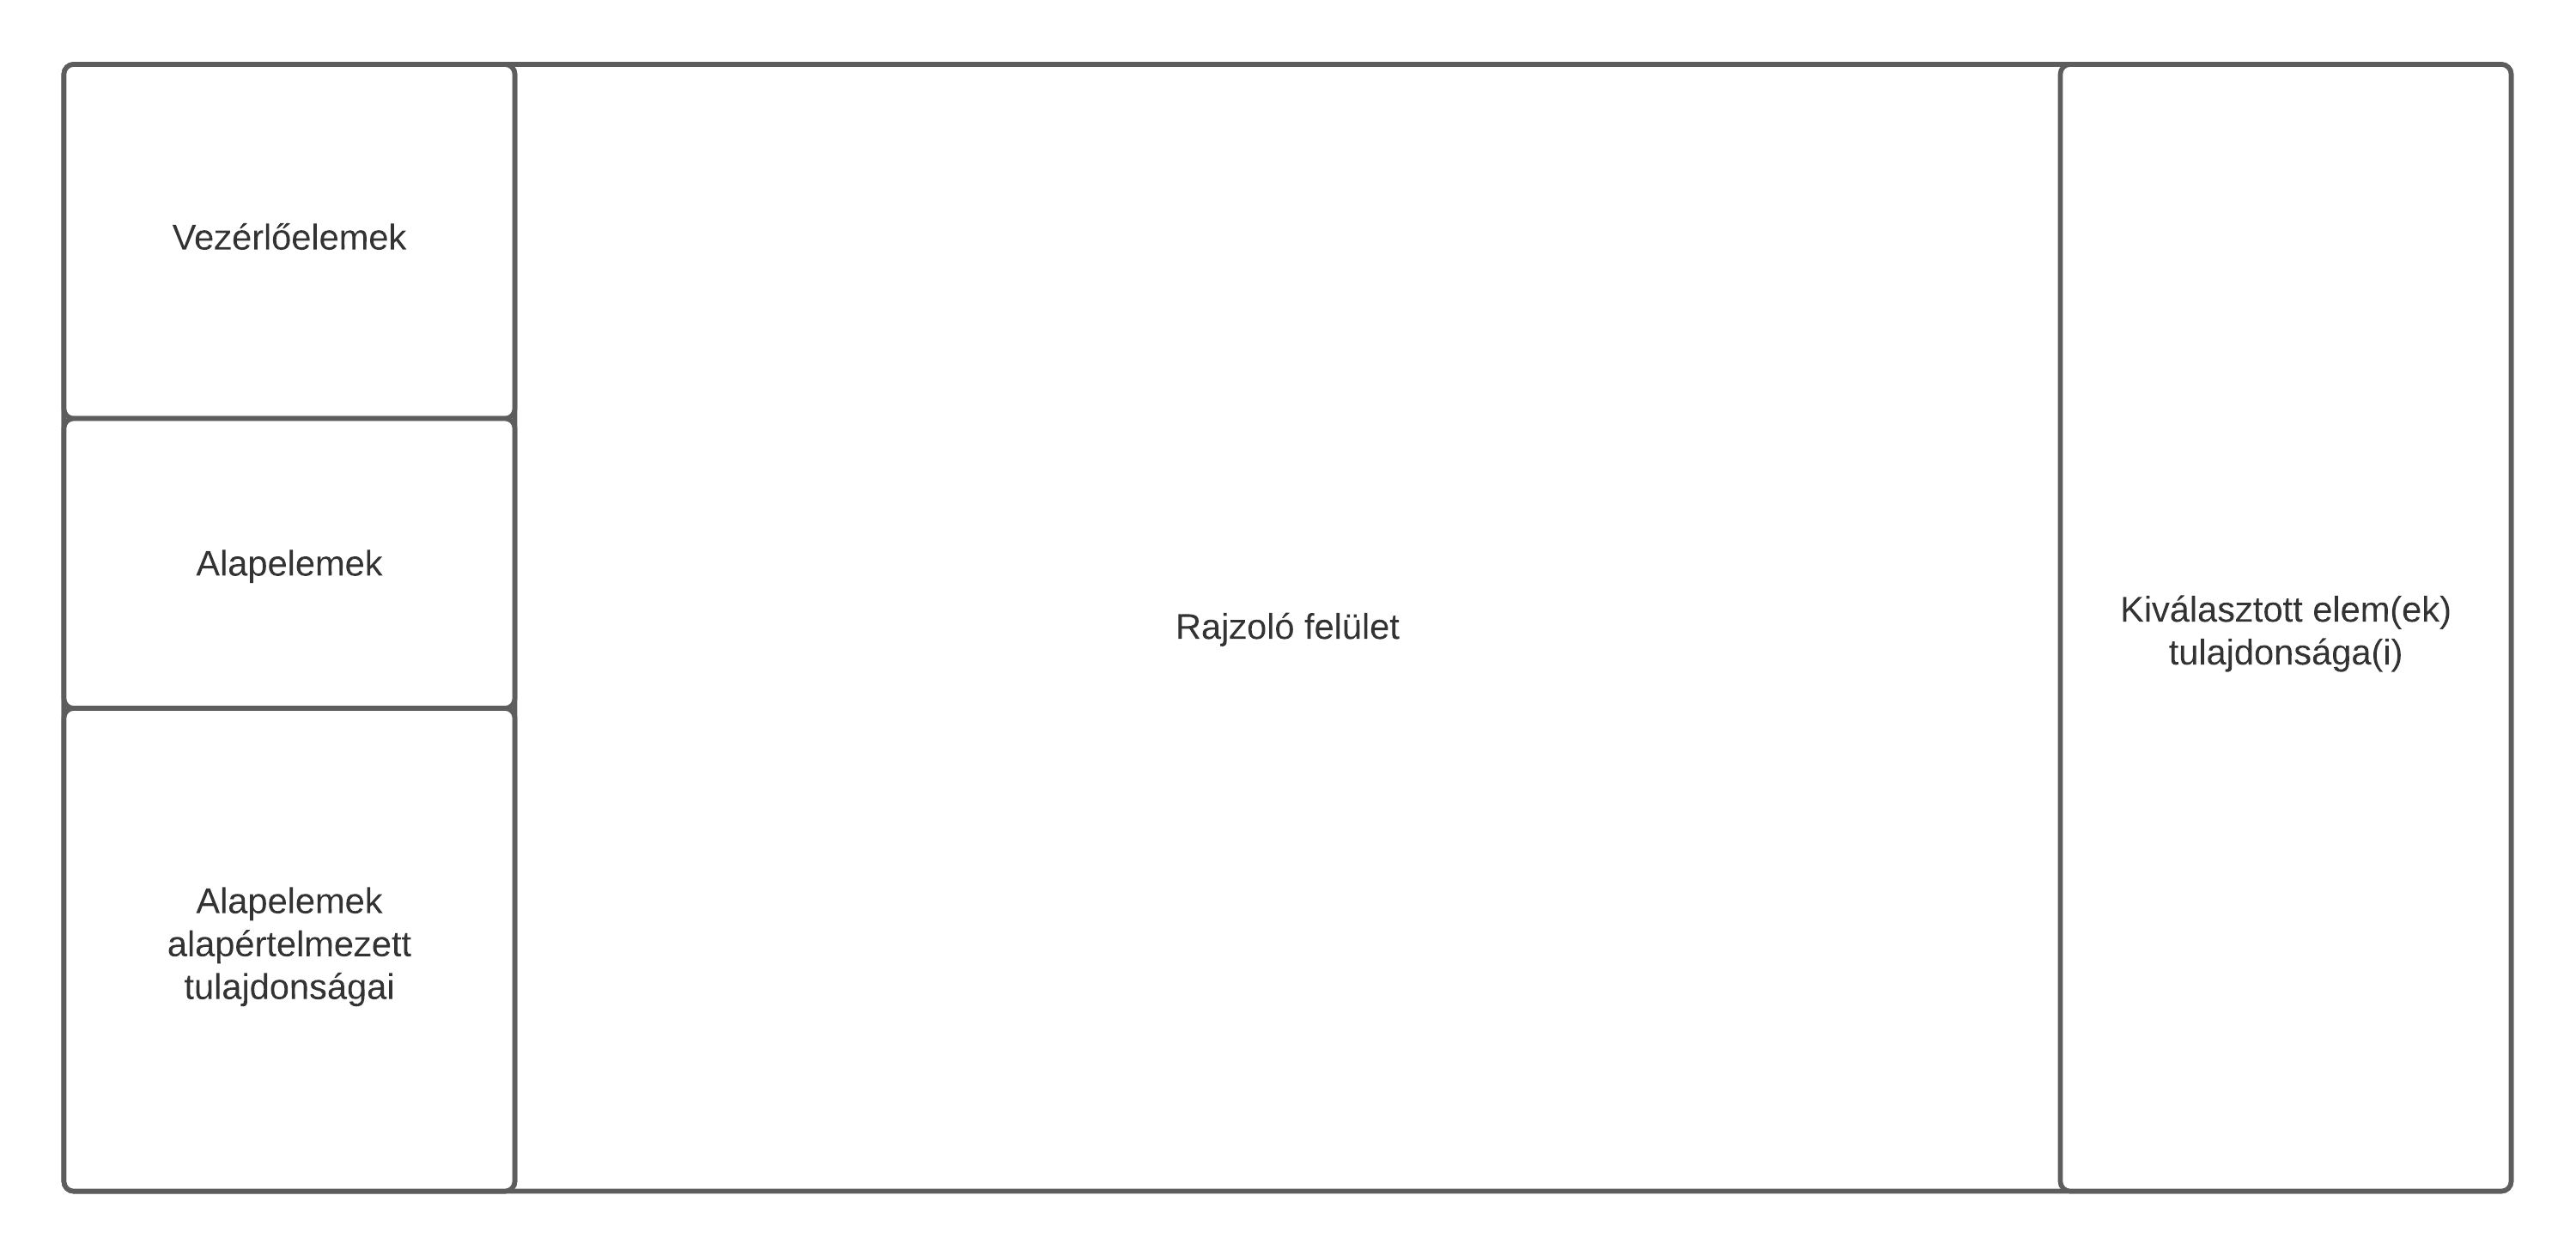
\includegraphics[width=\textwidth]{images/block.png}
	\caption{Az alkalmazás felépítése}
	\label{fig:block}
\end{figure}

Az alkalmazás legyen reszponzív akár a felület, akár a funkciók megjelenítése szempontjából. A reszponzív webdesign egy újabb megközelítés, amely a \textit{CSS3}-on és a \textit{CSS @media} szabály továbbfejlesztett használatán keresztül az oldal stíluslapján belül a készülékenkénti specifikáció mélyebb szintjén alapul. 

\Section{Alapelemek megjelenítése, és kiválasztása}

Az alapelemek megjelenése és kiválasztása egyaránt fontos a felhasználó megragadásában. Ha ezek átláthatók, és jól használhatók, akkor nagyobb célközönséghez juthat el az alkalmazásunk.

\SubSection{Alapelemek megjelenítése}

A funkciók a weboldal első hasábját foglalja magába, itt találhatók meg az alapelemek is a vezérlőelemeken és a kiválasztott elem tulajdonságainak kiválasztásán felül.  

Az alkotóelemek a kis hely miatt két oszlopban lelhetők fel, tehát az alkalmazás mátrix alapú elrendezést használ. Célszerű az elemeket csoportosítani olyan tulajdonságok alapján, amiben megegyeznek: például a vonal és a görbe jelenleg meg egymás mellett a mátrixban. 

\SubSection{Alapelemek kiválasztása}

A rajzolási mód kiválasztása után automatikusan ki legyen választva a mátrix első eleme, mint aktuális elem. Az alapelemek kiválasztása a mátrix alapú listában történik beavatkozással. A felhasználó egérrel kiválasztja a számára szükséges elemet. A kiválasztás után megjelenik az adott elemekhez tartozó tulajdonságok listája, amivel ezek módosíthatók is.

\Section{Tulajdonságok szerkesztési lehetőségei}

A tulajdonságok szerkesztése szintén fontos akár az új, akár a meglévő elemek tulajdonságait szeretnénk módosítani. A felhasználó nem feltétlenül csak fekete-fehér ábrákat szeretne szerkeszteni.

\SubSection{Új elemek esetében}

Új elemek esetében minden újonnan lerakott elemre érvényesüljön az itt megadott beállítás. Ez érinti az elemek színét, kitöltési színét, vonal vastagságát és mintázatát is. Az elemek kezdeti és végpontjai kattintásra kerülnek a vászonra. Ahol szükséges egyéb tulajdonság is, mint például körvonal esetében a kezdő és végszögek külön beírhatók legyenek.

\SubSection{Meglévő elemek esetében}

A már lent lévő elemek esetében kijelölés után minden tulajdonságnak szerkeszthetőnek kell lennie. Ehhez a szerkesztő jobb oldalán lévő hasáb ad majd helyet. A kijelölt elemek meglévő tulajdonságait be kell tölteni, és változtatás esetén az adott elem tulajdonságait ez alapján módosítani. Fontos, hogy csak a releváns tulajdonságok jelenjenek meg.

\Section{Színek megadási módjai}

A szerkesztőnek tudnia kell kezelni a színeket, és ezeknek kiválaszthatónak kell lenniük. Az \LaTeX\ által előre definiált színeket elérhetővé kell tenni a felhasználónak. 

A színek kiválasztásához célszerű valamilyen lenyíló menüt használni, ezzel megkönnyítve ezeknek az elérését. 

\begin{figure}[!h]
	\centering
	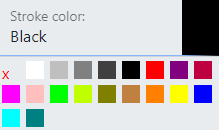
\includegraphics[]{images/colorpicker.png}
	\caption{Példa a színek kiválasztására}
	\label{fig:cp}
\end{figure}

Ebben az esetben megjelenítésre kerül a módosított tulajdonság, a kiválasztott szín, és a választható színek egyaránt. Az első elem a címek között jelöli azt, amikor nem kerül szín kiválasztásra: használható a körvonal eltüntetésére, vagy az ábra fehérrel történő kitöltés elkerülésére.

\Section{Objektumok automatikus igazítása}

Az alkalmazásnak tudnia kell kezelni a rácspontokat, és az ábrák egyes pontjait ezekhez kell igazítania. Az igazításnak meg kell történni ábra lerakásakor és már lent lévő elem kezdeti és végpontjai módosításakor. A Bézier-görbe esetében a kontrollpontok szintén paraméteresen módosíthatónak kell lenniük.

\Section{Objektumok összekapcsolási módjai}

A szerkeszthetőség érdekében lehetőséget kell adni a felhasználónak a már lent lévő objektumok összekapcsolására. Az összekapcsolás legegyszerűbb módja a pontok rácspontokhoz kapcsolása, és a kijelölés során lehetőséget adni több elem kijelölésére. Ebben az esetben a kijelölt pontok összekapcsolódnak, és mozgatásra együtt kerülnek kiszámolásra.

\Section{Szövegek szerkesztése}

Az alkalmazásnak kezelni kell a szöveget. A szövegeknek a vászonra lerakhatóknak és utólag szerkeszthetőeknek kell lenniük. 

A szövegekbe beletartoznak a \LaTeX\ matematikai módban írt kifejezései is, tehát például az $$ \int_{a}^{b} \qquad\qquad \bigcap_{a}^{b} \qquad\qquad \bigcup_{a}^{b} \qquad\qquad \sum_{a}^{b} \qquad\qquad \prod_{a}^{b}$$ kifejezéseknek meg kell tudnia jelenni.

\Section{Kijelölés}

Az alkalmazásnak lehetővé kell tenni az elemek kijelölését. A kijelöléshez egérbillentyűket kell használni. A kijelölés után az adott elemek tulajdonságait módosítani lehet, másolni, és törölni. 

 Téglalap alapú kijelölés esetén egyszerre több elem is kijelölhető, még a kattintás alapú kijelölés esetén egy kattintással csak egy elem jelölhető ki, esetleg funkciógombokkal (mint például a \textit{CTRL}, vagy az \textit{ALT} billentyű) van lehetőség több elemet kijelölni.

\Section{Másolás és beillesztés}

A "\textit{másolás és beillesztés}" kifejezés a szöveg vagy más adatok forrásból a célba történő másolásának népszerű, egyszerű módszerére utal. A módszer népszerűsége az egyszerűségéből ered, valamint abból, hogy a felhasználók vizuálisan - állandó tárolás nélkül - könnyen mozgathatják az adatokat a különböző alkalmazások között. Miután adatokat másoltunk a vágólapra, a vágólap tartalmát beilleszthetjük a céldokumentumba.

\SubSection{Másolás}

A kijelölt elemek másolása billentyű lenyomásra működjön, megszokott alapon a \textit{C} billentyűre vagy a \textit{CTRL + C} billentyűkombinációra. A kijelölt elemek tulajdonságai (pozíció, szín, kitöltési szín...) kerüljenek mentésre egyaránt. 

\SubSection{Beillesztés}

A másolt elemek beillesztése szintén billentyű lenyomásra működjön, megszokott alapon a \textit{V} billentyűre vagy a \textit{CTRL + V} billentyűkombinációra. 

A beillesztett elemek ne a másolt elemeken, hanem kicsit eltolva jelenleg meg az átláthatóság és könnyebb szerkeszthetőség érdekében.

\Section{Kicsinyítés és nagyítás}

Az oldal nagyításának két különböző módja van:

\begin{itemize}
	\item a szövegek átméretezése a betűméret növelésével vagy csökkentésével, a vízszintes görgetés elkerülése érdekében a képek méretének változatlanul hagyásával.
	\item valódi átméretezés, amely a képeket, egyéb multimédiás objektumokat és a nézetablakokat is átméretezi.
\end{itemize}

Az alkalmazásnak támogatnia kell a kicsinyítését és nagyítását, legalább a vásznon megjelenő alapelemek méretének nagyításával vagy csökkentésével. Ezt célszerű az egér görgőjére hivatkozva módosítani: ha felfelé görgetünk, akkor nagyítsuk a vásznak, ellenkező esetben kicsinyítjük.

\Section{Undo-redo funkciók}

Az elkészült alkalmazásnak biztosítani kell a visszavonás és az újra lerakás funkcióit. Sokszor fordul az elő, hogy a felhasználó véletlenül más elemet rajzol a vászonra, vagy esetleg más elem tulajdonságait módosítja, így a felhasználói élmény növelése céljából szükség van ezeknek a hibáknak a visszavonására.

\Section{Mentés, és automatikus mentés}

\SubSection{Mentés}

Mentés során a felhasználó megkapja a szerkesztett ábrát \LaTeX\-be visszailleszthető állapotba. Ez egyaránt jelenti a \LaTeX\ kódot, valamint egy opcionálisan letölthető \textit{.tex} formátumú fájlt, amely az \textit{input} paranccsal betölthető tetszőleges \LaTeX\ állományba.

A mentés során a felhasználó kap egy hivatkozási kódot is, amely a későbbi betöltéshez szükséges. Ez egy \textit{BASE64} kódolású szöveg lenne, amelynek az a jelentősége, hogy elfedje a háttérben lévő "adatbázist", amelyből a kimentéshez szükséges \textit{JSON} objektumot kapjuk.

\SubSection{Automatikus mentés}

Az automatikus mentés számos számítógépes alkalmazás és videojáték mentési funkciója, amely automatikusan elmenti a program vagy játék aktuális változásait vagy előrehaladását, így segít csökkenteni az adatvesztés kockázatát vagy hatását összeomlás, lefagyás vagy felhasználói hiba esetén. Az automatikus mentés jellemzően vagy előre meghatározott időközönként, vagy egy összetett szerkesztési feladat megkezdése előtt, közben és után történik. Hagyományosan olyan funkciónak tekintették, amely alkalmazás- vagy rendszerhiba (például összeomlás) esetén védi a dokumentumokat, és az automatikus mentéses biztonsági mentéseket gyakran törlik, amikor a felhasználó befejezi a munkáját. A megvalósítás a fájl, az alkalmazás és az operációs rendszer szintjén is kihívásokkal jár.

Ezek alapján az alkalmazásnak támogatnia kell az automatikus mentés funkciót. A legegyszerűbb megvalósítása ennek a fix időközönkénti állapotmentés. Web alkalmazás révén ehhez a megoldás a \textit{HTTP-süti}k használata.

A HTTP-sütik (vagy más néven böngészősütik vagy egyszerűen sütik) olyan kis adatblokkok, amelyeket egy webszerver hoz létre, miközben a felhasználó egy webhelyet böngészik, és amelyeket a  webböngésző helyez el a felhasználó számítógépén vagy más eszközén. A sütik a weboldal eléréséhez használt eszközön kerülnek elhelyezésre, és egy munkamenet során egynél több süti is elhelyezhető a felhasználó eszközén.





